%\documentclass[pdf]{beamer}
\documentclass[aspectratio=169]{beamer}
% \documentclass[pdf,aspectratio=169]{beamer} % Template is not ready for 16:9
\usepackage{graphicx}
\usepackage{listings}
\usepackage{amsmath}
\usepackage{epsfig}
\usepackage{epstopdf}
\usepackage{xspace}
\usepackage{tikz}
\usepackage{xcolor}
\usepackage{colortbl}
\usepackage{shortcuts}
% \usepackage{framed}
\usepackage{multirow}
\usepackage{colortbl}
\usepackage{subcaption}
\usepackage{minted}
\usepackage{rotating}
\usepackage[]{hyperref}
 \hypersetup{
    colorlinks = true,
    linkcolor = red,
    anchorcolor = blue,
    citecolor = blue,
    filecolor = blue,
    urlcolor = blue
}


 \makeatletter
\setbeamercolor{headline}{fg=black,bg=black}
\setbeamercolor{section in head/foot}{bg=gray}

\setbeamertemplate{headline}{%
    \begin{beamercolorbox}[ht=2.25ex,dp=3.75ex]{section in head/foot}
        \insertnavigation{\paperwidth}
     \end{beamercolorbox}%
}%
\makeatother

\usepackage[nomessages]{fp}% http://ctan.org/pkg/fp
\newcommand{\maxnum}{100.00}
\newlength{\maxlenA}
\newcommand{\databar}[2][red!25]{%
  \settowidth{\maxlenA}{\maxnum}%
  \addtolength{\maxlenA}{\tabcolsep}%
  \FPeval\result{round(#2/\maxnum:4)}%
  \rlap{\color{red!25}\hspace*{-.5\tabcolsep}\rule[-.05\ht\strutbox]{\result\maxlenA}{.95\ht\strutbox}}%
  \makebox[\dimexpr\maxlenA-\tabcolsep][r]{#2}%
}

\newcommand{\maxnumApp}{4000.00}
\newlength{\maxlenB}
\newcommand{\databarApp}[3][red!25]{%
  \settowidth{\maxlenB}{\maxnumApp}%
  \addtolength{\maxlenB}{\tabcolsep}%
  \FPeval\result{round(#2/\maxnumApp:4)}%
  \rlap{\color{red!25}\hspace*{-.5\tabcolsep}\rule[-.05\ht\strutbox]{\result\maxlenB}{.95\ht\strutbox}}%
  \makebox[\dimexpr\maxlenB-\tabcolsep][r]{#3}%
}

\newcommand{\maxnumJW}{3000.00}
\newlength{\maxlenC}
\newcommand{\databarJW}[3][red!25]{%
  \settowidth{\maxlenC}{\maxnumJW}%
  \addtolength{\maxlenC}{\tabcolsep}%
  \FPeval\result{round(#2/\maxnumJW:4)}%
  \rlap{\color{red!25}\hspace*{-.5\tabcolsep}\rule[-.05\ht\strutbox]{\result\maxlenC}{.95\ht\strutbox}}%
  \makebox[\dimexpr\maxlenC-\tabcolsep][r]{#3}%
}

\newcommand{\maxnumNC}{400.00}
\newlength{\maxlenD}
\newcommand{\databarNC}[3][red!25]{%
  \settowidth{\maxlenD}{\maxnumNC}%
  \addtolength{\maxlenD}{\tabcolsep}%
  \FPeval\result{round(#2/\maxnumNC:4)}%
  \rlap{\color{red!25}\hspace*{-.5\tabcolsep}\rule[-.05\ht\strutbox]{\result\maxlenD}{.95\ht\strutbox}}%
  \makebox[\dimexpr\maxlenD-\tabcolsep][r]{#3}%
}

\newcommand{\maxnumHC}{400.00}
\newlength{\maxlen}
\newcommand{\databarHC}[3][red!25]{%
  \settowidth{\maxlen}{\maxnumHC}%
  \addtolength{\maxlen}{\tabcolsep}%
  \FPeval\result{round(#2/\maxnumHC:4)}%
  \rlap{\color{red!25}\hspace*{-.5\tabcolsep}\rule[-.05\ht\strutbox]{\result\maxlen}{.95\ht\strutbox}}%
  \makebox[\dimexpr\maxlen-\tabcolsep][r]{#3}%
}

% \newcommand{\ttt}[1]{\texttt{\justify #1}}
\newcommand{\ttt}[1]{\texttt{#1}}
\newcommand{\hl}[1]{\textcolor{utdorange}{\textbf{#1}}}
\newcommand{\bm}{BigMatrix}
\usetheme{default}

\setbeamertemplate{note page}[plain]
%\useoutertheme{infolines}
%\usepackage[all,knot]{xy}
%\xyoption{arc}
\usepackage{url}
%\usepackage{multimedia}
\usepackage{hyperref}
\usepackage{colortbl}

\usepackage[normalem]{ulem}

\usepackage{epsfig}
\usepackage{shortcuts}
\usepackage{pgfplots}
\usepackage{tikz}
%\usepackage{amsfonts}
\newcommand{\tickYes}{\checkmark}
\usepackage{pifont}
\newcommand{\tickNo}{\hspace{1pt}\ding{55}}
\newcommand{\Yes}{\ding{52}}
\newcommand{\No}{\ding{55}}
\usepackage{wasysym}
\newcommand{\yes}{\CIRCLE}
\newcommand{\no}{\Circle}
\usepackage{graphicx}
\newcommand{\infi}{$\infty$}

\usepackage{booktabs}

% Standard packages
%
%\usepackage[english]{babel}
%\usepackage[latin1]{inputenc}
%\usepackage{times}
%\usepackage[T1]{fontenc}
%
%\usepackage{animate}
%\usepackage{ulem}

%%%
\usetikzlibrary{shapes,arrows}
%\tikzstyle{block}=[draw opacity=0.7,line width=1.4cm]
% Define block styles
\tikzstyle{decision} = [diamond, draw, fill=blue!20, 
    text width=4.5em, text badly centered, node distance=3cm, inner sep=0pt]
\tikzstyle{block} = [rectangle, draw, fill=blue!20, 
    text width=3em, text centered, rounded corners, minimum height=2em]
\tikzstyle{line} = [draw, -latex']
\tikzstyle{cloud} = [draw, ellipse,fill=red!20, node distance=3cm,
    minimum height=2em]


\newcommand*\circled[1]{\tikz[baseline=(char.base)]{\tiny \node[shape=circle,draw,inner sep=1pt] (char) {#1};}}


% \newcommand{\ttt}[1]{\texttt{\justify #1}}
 
 
 
\newcommand{\sysname}{{\sc FirmXRay}\xspace}
\newcommand{\leakscope}{{\sc LeakScope}}
\newcommand{\smartgen}{{\sc SmartGen}}
\newcommand{\authscope}{{\sc AuthScope}}

%%%%%%%%%%%%
\ignore{
\AtBeginSection[] {
  \begin{frame}[plain]
    \frametitle{Outline}
    \tableofcontents[currentsection]
  \end{frame}
  \addtocounter{framenumber}{-1}
}

\AtBeginSubsection[] {
  \begin{frame}[plain]
   \frametitle{Outline}
    \tableofcontents[currentsubsection]
    \addtocounter{framenumber}{-1}
  \end{frame}
}
}
%%%%%%%%%%%
 
%\subtitle{ACM Symposium on Cloud Computing}
\setbeamertemplate
 {footline}{\quad\hfill\insertframenumber/\inserttotalframenumber\strut\quad} 
\bigskip

\title{\bf{ {\LARGE \\ MATH 100:\\Linear Algebra}}}

\author{\normalsize {\bf Lecture 1}}
\medskip


\author{ Yuqing Yang\\Assistant Professor\\School of Computer Science and Engineering\\
\smallskip
%ACM CCS 2022\\
% {\large 08/10/2020}
\medskip
%\small{Joint work w/ Haohuang Wen, Yinqian Zhang, and Chaoshun Zuo}\\
%\bigskip
\medskip
{\small 09/02/2026}
}





%\institute[shortinst]{%
%%    The Ohio State University %
    
%}

% \institute{\normalsize Department of Computer Science and Engineering \\ The Ohio State University}

\date{}%\footnotesize{CCS 2022}}




\mode<presentation>
{
    \usetheme{OSUCSE169}
    \setbeamercovered{transparent = 28}
}

%\renewcommand{\inserttotalframenumber}{21}
  \setbeamertemplate{footline}[frame number]


% \setbeamertemplate
% {footline}{\quad\hfill\insertframenumber/\inserttotalframenumber\str%ut\quad} 



\begin{document}
 
\setbeamercovered{invisible}

{
 
   %\titlepagebackground
    \usebackgroundtemplate{
\includegraphics[width=\paperwidth]{template-images/osuseclab169.pdf}}%
   \thispagestyle{empty}
    \frame[noframenumbering]{\titlepage  }

}

% \title{{\sc PT\_CFI}: Practical Backward-Edge Control Flow Integrity Using Intel Processor Trace}

 



%page 2
%---------------------------------------------------------------------

\section{Introduction}
\subsection{}
\begin{frame}{About me}

\end{frame}

\begin{frame}{Research and Services}

\end{frame}

\begin{frame}{Course and Office Hour Schedule}
  May need to adjust two instances of course

\end{frame}


\begin{frame}{Policies}
Teaching is fulily English, QA can be Chinese

How to reach me

Course policy
\end{frame}

\section{Introduction}

\begin{frame}{Language}
  Mathematical Language
  A set of properties
  Do not remember what it is. Remember why we have them, and what we can use with them
\end{frame}

\begin{frame}{Our world as a system: Game Movement}
  GTA
\end{frame}

\begin{frame}{Our world as a system: Pipeline Building}
  Endfield
\end{frame}

\begin{frame}{Our world as a system: Computer Graphics}

\end{frame}


\begin{frame}{AI model: parallel and sequential}
  Linear Algebra build what we are today
\end{frame}


\section{}
\subsection{Three Views of Linear Systems}
\begin{frame}{Ultimate Goal of Linear Algebra}
  We want to solve a system of equations:
  \[
  \begin{cases}
    x_1 + 2x_2 = 5 \\
    2x_1 + 3x_2 = 8
  \end{cases}
  \]
  where:
  \begin{itemize}
    \item \textbf{Equation}: mathematical statement that asserts the equality of two expressions
    \item \textbf{System}: a collection of one or more equations involving the same set of variables
    \item \textbf{Solution}: find all values of the unknowns that satisfy every equation in the system
  \end{itemize}
\end{frame}

\begin{frame}{Example}
  Consider the system with 2 equations and 2 unknowns:
  \[
  \begin{cases}
  2x - y = 0 \\
  -x + 2y = 3
  \end{cases}
  \]
  This system has the matrix form:
  \[
  \begin{bmatrix}
  2 & -1 \\
  -1 & 2
  \end{bmatrix}
  \begin{bmatrix}x \\ y\end{bmatrix}
  =
  \begin{bmatrix}0 \\ 3\end{bmatrix}
  \]
  \smallskip
  The coefficient matrix is $A$, the unknown vector is $\mathbf{x}$, and the right-hand side is $\mathbf{b}$.
\end{frame}

\begin{frame}{Example cont.}
  Keep the same equations, but look at them in three different ways:
  \begin{itemize}
    \item \textbf{Row picture}: each equation is a line in the plane
    \item \textbf{Column picture}: the solution is a combination of column vectors
    \item \textbf{Matrix picture}: write everything in compact linear algebra form
  \end{itemize}
  These viewpoints are equivalent, but each gives a different intuition.
\end{frame}

\begin{frame}{Row picture}
  \begin{columns}[T,onlytextwidth]
    \column{0.35\textwidth}
    \begin{itemize}
      \item $2x-y=0$
      \item $-x+2y=3$
    \end{itemize}

    \column{0.65\textwidth}
    \centering
    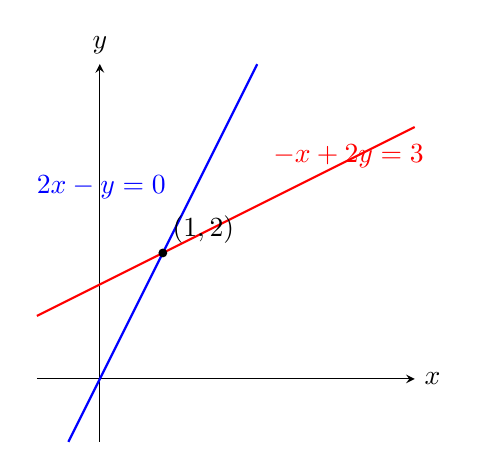
\begin{tikzpicture}[scale=0.8,>=stealth]
      \draw[->] (-1,0) -- (5,0) node[right] {$x$};
      \draw[->] (0,-1) -- (0,5) node[above] {$y$};

      % line 2x - y = 0  =>  y = 2x
      \draw[blue,thick,domain=-0.5:2.5,samples=100] plot (\x,{2*\x});
      % line -x + 2y = 3 => y = (x+3)/2
      \draw[red,thick,domain=-1:5,samples=100] plot (\x,{(\x+3)/2});

      % intersection point
      \fill (1,2) circle (2pt);
      \node[above right] at (1,2) {$(1,2)$};

      \node[above left,blue] at (1.2,2.7) {$2x-y=0$};
      \node[above right,red] at (2.6,3.2) {$-x+2y=3$};
    \end{tikzpicture}
  \end{columns}
\end{frame}

\begin{frame}{Column picture}
  \begin{columns}[T,onlytextwidth]
    \column{0.42\textwidth}
    The same system can be written as a linear combination of vectors:
    \[
    1\begin{bmatrix}2 \\ -1\end{bmatrix}
    +
    1\begin{bmatrix}-1 \\ 2\end{bmatrix}
    =
    \begin{bmatrix}1 \\ 1\end{bmatrix}
    \]

    \smallskip

    \column{0.58\textwidth}
    \centering
    \begin{tikzpicture}[scale=1.1,>=stealth]
      \draw[->] (-2,0) -- (3,0) node[right] {$x$};
      \draw[->] (0,-2) -- (0,3) node[above] {$y$};

      % black vectors
      \draw[black, thick, ->] (0,0) -- (2,-1) node[below right] {$\begin{bmatrix}2\\-1\end{bmatrix}$};
      \draw[black, thick, ->] (0,0) -- (-1,2) node[above left] {$\begin{bmatrix}-1\\2\end{bmatrix}$};

      % red target vector
      \draw[red, thick, ->] (0,0) -- (1,1) node[above right, text=red] {$\mathbf{b}$};

      % dotted connection lines
      \draw[dotted, black, thick] (2,-1) -- (1,1);
      \draw[dotted, black, thick] (-1,2) -- (1,1);
    \end{tikzpicture}
  \end{columns}
\end{frame}

\begin{frame}{Column picture}
  \begin{columns}[T,onlytextwidth]
    \column{0.42\textwidth}
    \[
    x\begin{bmatrix}2 \\ -1\end{bmatrix}
    +
    y\begin{bmatrix}-1 \\ 2\end{bmatrix}
    =
    \begin{bmatrix}2x-y \\ -x+2y\end{bmatrix}
    \]

    \smallskip
    $$x=0.5$$
    
    $$y=1$$
    \column{0.58\textwidth}
    \centering
    \begin{tikzpicture}[scale=0.8,>=stealth]
      \draw[->] (-2,0) -- (3,0) node[right] {$x$};
      \draw[->] (0,-3) -- (0,4) node[above] {$y$};

      % black vectors
      \draw[black, thick, ->] (0,0) -- (2,-1) node[below right] {$\begin{bmatrix}2\\-1\end{bmatrix}$};
      \draw[black, thick, ->] (0,0) -- (-2,4) node[above left] {$\begin{bmatrix}-2\\4\end{bmatrix}$};

      % red target vector
      \draw[red, thick, ->] (0,0) -- (0,3) node[above right, text=red] {$\mathbf{b}$};

      % dotted connection lines
      \draw[dotted, black, thick] (2,-1) -- (0,3);
      \draw[dotted, black, thick] (-2,4) -- (0,3);
    \end{tikzpicture}
  \end{columns}
\end{frame}


\begin{frame}{Column picture}
  \begin{columns}[T,onlytextwidth]
    \column{0.38\textwidth}
    \textbf{Now: what is the combination of x and y?}
    \smallskip

    $$x=1$$


    $$y=2$$
    \column{0.62\textwidth}
    \centering
    \begin{tikzpicture}[scale=0.8,>=stealth]
      \draw[->] (-2,0) -- (3,0) node[right] {$x$};
      \draw[->] (0,-3) -- (0,4) node[above] {$y$};

      % translated vectors
      \draw[black, thick, ->] (0,0) -- (2,-1) node[below right] {$1\begin{bmatrix}2\\-1\end{bmatrix}$};
      \draw[black, thick, ->] (0,0) -- (-2,4) node[above left] {$2\begin{bmatrix}-1\\2\end{bmatrix}$};

      % vector b
      \draw[red, thick, ->] (0,0) -- (0,3) node[above right, text=red] {$\mathbf{b}$};
      \fill[red] (0,0) circle (2pt);
      \node[below left, red] at (-2,-1) {start $=(0,0)$};
      \node[above right, red] at (1,3) {end $=(0,3)$};

        \draw[dotted, black, thick] (2,-1) -- (0,3);
      \draw[dotted, black, thick] (-2,4) -- (0,3);
    \end{tikzpicture}
  \end{columns}
\end{frame}

\begin{frame}{Matrix}
  \begin{columns}[T,onlytextwidth]
    \column{0.48\textwidth}
\begin{center}
  \[
    \begin{bmatrix}
      2 & -1\\
      -1 & 2
    \end{bmatrix}
    \begin{bmatrix}
      x\\
      y
    \end{bmatrix}
    =
    \begin{bmatrix}
      0\\
      3
    \end{bmatrix}
  \]
\\
  \[
    \begin{array}{cc|c}
      2 & -1 & 0\\
      -1 & 2 & 3
    \end{array}
  \]
  \[
    \begin{array}{cc|c}
      2 & -1 & 0\\
      0 & 3 & 6
    \end{array}
  \]
\end{center}
    \column{0.48\textwidth}
  \end{columns}
\end{frame}


% Cover the idea of:
% Linear 
% Definition: at most power of 1 
% Properties: preserving multiplication/addition)

% Overview
% Input -> System -> Output
% Solution: existence, uniqueness, solution

% Determinants 
% Vector Spaces

% Representation: Eigenvalues and Eigenvectors
% Approximation: Least Square

\subsection{Linear Combination}
\begin{frame}{Why do they work?}
  Linear
\end{frame}

\begin{frame}{Okay, define linear for me.}
  Book
  Ours
\end{frame}

\begin{frame}{Tricky. How to I tell?}
  A function is linear if it satisfies two properties:
  \begin{itemize}
    \item Additivity: $f(x + y) = f(x) + f(y)$
    \item Homogeneity: $f(cx) = c f(x)$
  \end{itemize}
\end{frame}

\begin{frame}{In the form of matrix...}
  Let
  \[
    A = \begin{pmatrix} 1 & 2 \\ 3 & 4 \end{pmatrix}, \qquad
    B = \begin{pmatrix} 5 & -1 \\ 0 & 2 \end{pmatrix}.
  \]
  Preserving Addition:
  \[
    A + B =
    \begin{pmatrix} 1+5 & 2+(-1) \\ 3+0 & 4+2 \end{pmatrix}
    = \begin{pmatrix} 6 & 1 \\ 3 & 6 \end{pmatrix}.
  \]
  Preserving Multiplication:
  \[
    3A = 3\begin{pmatrix} 1 & 2 \\ 3 & 4 \end{pmatrix}
       = \begin{pmatrix} 3 & 6 \\ 9 & 12 \end{pmatrix}.
  \]
\end{frame}

\subsection{Existence of Solutions}
\begin{frame}{How many solutions can there be?}
  one
  unlimited
  none
\end{frame}

\begin{frame}{Three examples}
  
\end{frame}

\begin{frame}{Existence of Solutions}
  Consistent vs Equivalent
\end{frame}


\begin{frame}{"Good" matrix}
  M x N
  N x N
\end{frame}


\begin{frame}{Pre:Order of Matrix}
  "Enough" equations and "Just Enough" equations
  Simplified form (reduce equivalent)
\end{frame}
\subsection{Elimintation}
\begin{frame}{}

\end{frame}
\begin{frame}{Elementary Row Operations}
  Interchange
  Scaling
  Replacement (Addition)
\end{frame}

\begin{frame}{Practice: into echelon form}
\end{frame}
\begin{frame}{What does echelon form look like}
\end{frame}

\begin{frame}{Terminologies}
  nonzero
  pivot
  pivot column
  pivot row
  "I am a pivot student" ---> I hope you are all nonzero students...
\end{frame}

\begin{frame}{Elementary Row Reduction}
\end{frame}
\begin{frame}{Leading variable and free variable}
\end{frame}
\begin{frame}{Existence and Uniqueness}
\end{frame}
\begin{frame}{Gaussian Elimination}
\end{frame}

% End of 1.1

% 1.2 Row reduction
% overdetermined and underdetermined
% Rank of a matrix
% Determine the solutioin amount

\begin{frame}{}
\end{frame}

\begin{frame}{}
\end{frame}

\begin{frame}{}
\end{frame}

\begin{frame}{}
\end{frame}

\begin{frame}{}
\end{frame}


% \begin{frame}{Frame Title}
    
% \end{frame}
\end{document}
